\aufgabe 2

\todo{Patiiiii schau mal ob die Erklärungen für die Verifizierungen passen oder dass eher umgangssprachlich sein muss. Es ist spät und wir haben weder Lust noch nerven um das durchzudenken} 

\paragraph{a)}\mbox{} \\

\begin{figure}[H] 
	\centering 
	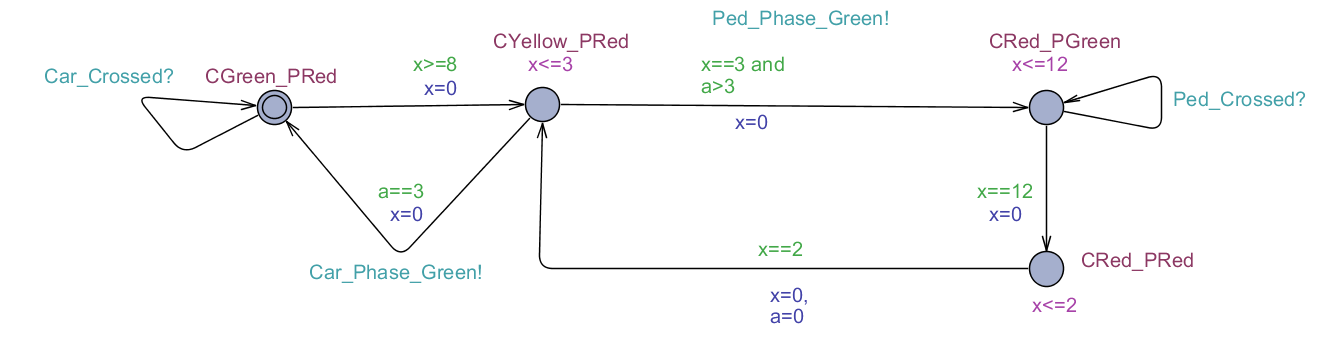
\includegraphics[width=\textwidth]{./UPAAAL_Screens/Contr1}
	\caption[Aufgabe 2a)]{Modell $Contr$ - Zum Zeitpunkt des Bildes wurden $Ped$ und $Car$ bereits erstellt}    
\end{figure}

\paragraph{b)}\mbox{} \\

%%BILD VON den Formeln 

\begin{figure}[H] 
	\centering 
	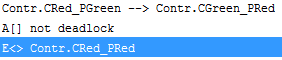
\includegraphics[width=0.5\textwidth]{./UPAAAL_Screens/2b_Verify}
	\caption[Aufgabe 2b)]{Entwickelte Properties zum Modell $Contr$}    
\end{figure}
%%BILD VOM ERGEBNIS der Formeln 

\begin{figure}[H] 
	\centering 
	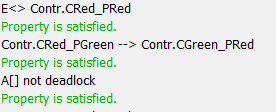
\includegraphics[width=0.5\textwidth]{./UPAAAL_Screens/2b_Ergebnisse}
	\caption[Aufgabe 2b)]{Verifizierungsergebnisse der oben angegebenen Properties}    
\end{figure}

Erklärung der Formeln für das Modell $Contr$:

\begin{enumerate}[i)]

	\item $E \left<\right> \text{Contr.CRed\_PRed} $\\
	Es existiert ein Pfad auf dem der Zustand $Contr.CRed\_PRed$ erreicht wird.
	
	\item $A[] \text{not deadlock}$ \\
	Es gibt keinen Deadlock innerhalb des Modells.
	
	\item $\text{Contr.CRed\_PGreen} \rightarrow  \text{Contr.CGreen\_PRed}$ \\
	Ausgehend vom Zustand $Contr.CRed\_PGreen$ wird irgendwann der Zustand $Contr.CGreen\_PRed$ erreicht.
	
\end{enumerate}

\paragraph{c)}\mbox{} \\

%%BILD PEDESTRIAN
\begin{figure}[H] 
	\centering 
	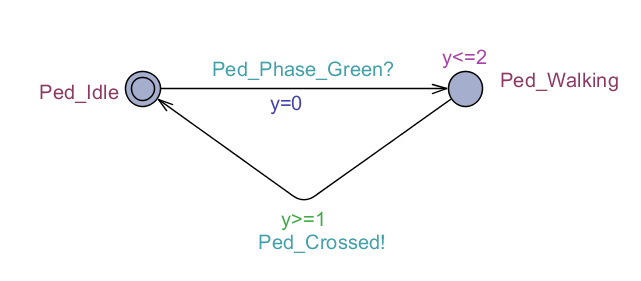
\includegraphics[width=0.6\textwidth]{./UPAAAL_Screens/Pedestrian}
	\caption[Aufgabe 2c)]{Modell $Ped$}    
\end{figure}

\paragraph{d)}\mbox{} \\

%%BILD Verifikation
\begin{figure}[H] 
	\centering 
	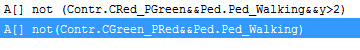
\includegraphics[width=0.5\textwidth]{./UPAAAL_Screens/2d_Verifyer}
	\caption[Aufgabe 2d)]{Entwickelte Properties zum Modell $Contr||Ped$}    
\end{figure}
%%BILD VOM ERGEBNIS der Formeln 

\begin{figure}[H] 
	\centering 
	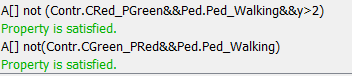
\includegraphics[width=0.5\textwidth]{./UPAAAL_Screens/2d_verifyer_Checkd}
	\caption[Aufgabe 2d)]{Verifizierungsergebnisse der oben angegebenen Properties}    
\end{figure}

Erklärung der Formeln für das Modell $Contr||Ped$

\begin{enumerate}[i)]
	
	\item $A \left[\right] \text{not} (\text{Contr.CRed\_PGreen} \&\& \text{Ped.Ped\_Walking} \&\& y>2)$\\
	Auf sämtlichen Pfaden gelten nicht gleichzeitig $Contr.CRed\_PGreen$ und $Ped.Ped\_Walking$ zu einem Zeitpunkt, an dem $y>2$ gilt.
	
	\item $A \left[\right] \text{not} (\text{Contr.CGreen\_PRed} \&\& \text{Ped.Ped\_Walking}) $\\
	Auf sämtlichen Pfaden gilt nicht gleichzeitig $Contr.CGreen\_PRed$ und $Ped.Ped\_Walking$.
\end{enumerate}




\paragraph{e)}\mbox{} \\

%%Bild Car automata
\begin{figure}[H] 
	\centering 
	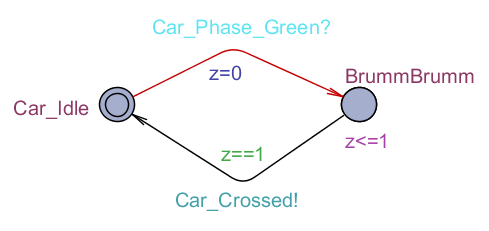
\includegraphics[width=0.5\textwidth]{./UPAAAL_Screens/Car}
	\caption[Aufgabe 2c)]{Modell $Car$}    
\end{figure}


\paragraph{f)}\mbox{} \\

%%BILD Verifikation
\begin{figure}[H] 
	\centering 
	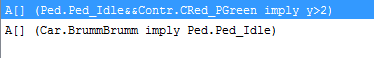
\includegraphics[width=0.5\textwidth]{./UPAAAL_Screens/2f_Verification}
	\caption[Aufgabe 2f)]{Entwickelte Properties zum Modell $Contr||Ped||Car$}    
\end{figure}
%%BILD VOM ERGEBNIS der Formeln 

\begin{figure}[H] 
	\centering 
	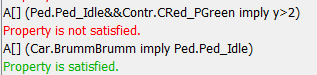
\includegraphics[width=0.5\textwidth]{./UPAAAL_Screens/2f_Verification_CHECKED}
	\caption[Aufgabe 2f)]{Verifizierungsergebnisse der oben angegebenen Properties}    
\end{figure}


Erklärung der Formeln für das Modell $Contr||Ped||Car$

\begin{enumerate}[i)]
	
	\item $A \left[\right]  (\text{Ped.Ped\_Idle} \&\& \text{Contr.CRed\_PGreen} \text{ imply } y>2)$ \\
	Auf sämtlichen Pfaden implizieren die gleichzeitig geltenden Zustände $Ped.Ped\_Idle$ und $Contr.CRed\_PGreen$, dass die Clock $y>2$ ist. 
	
	
	\item $A \left[\right] (\text{Car.BrummBrumm} \text{ imply } \text{Ped.Ped\_Idle}) $\\
	Auf sämtlichen Pfaden impliziert dass bei geltendem Zustand $Car.BrummBrumm$ ebenso $Ped.Ped\_Idle$.
	
\end{enumerate}


\paragraph{g)}\mbox{} \\
%%Verfiikation zu g 
\begin{figure}[H] 
	\centering 
	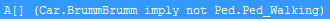
\includegraphics[width=0.5\textwidth]{./UPAAAL_Screens/2g_Formel}
	\caption[Aufgabe 2g)]{Zu überprüfunde Propertie des Modells $Contr||Ped||Car$}    
\end{figure}
%%BILD VOM ERGEBNIS der Formeln 

\begin{figure}[H] 
	\centering 
	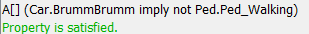
\includegraphics[width=0.5\textwidth]{./UPAAAL_Screens/2g-Verified}
	\caption[Aufgabe 2f)]{Verifizierungsergebnis der oben angegebenen Propertie}    
\end{figure}

\begin{enumerate}[i)]
	\item $A \left[\right] (\text{Car.BrummBrumm} \text{ imply not } \text{Ped.Ped\_Walking}) $\\
	Auf sämtlichen Pfaden impliziert der geltende Zustand $Car.BrummBrumm$ dass $Ped.Ped\_Walking$ ungültig ist.
\end{enumerate}

\paragraph{h)}\mbox{} \\

\begin{figure}[H] 
	\centering 
	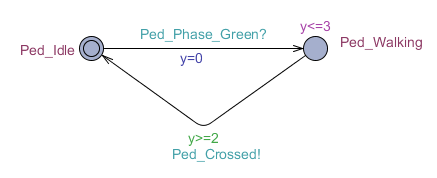
\includegraphics[width=0.6\textwidth]{./UPAAAL_Screens/2h_Graph}
	\caption[Aufgabe 2h)]{Modell $Ped$ mit langsameren Fußgänger}    
\end{figure} 

\begin{figure}[H] 
	\centering 
	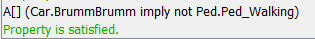
\includegraphics[width=0.5\textwidth]{./UPAAAL_Screens/2h_Verification}
	\caption[Aufgabe 2h)]{Verifizierungsergebnis der Propertie aus g)}    
\end{figure}

\paragraph{i)}\mbox{} \\

\begin{figure}[H] 
	\centering 
	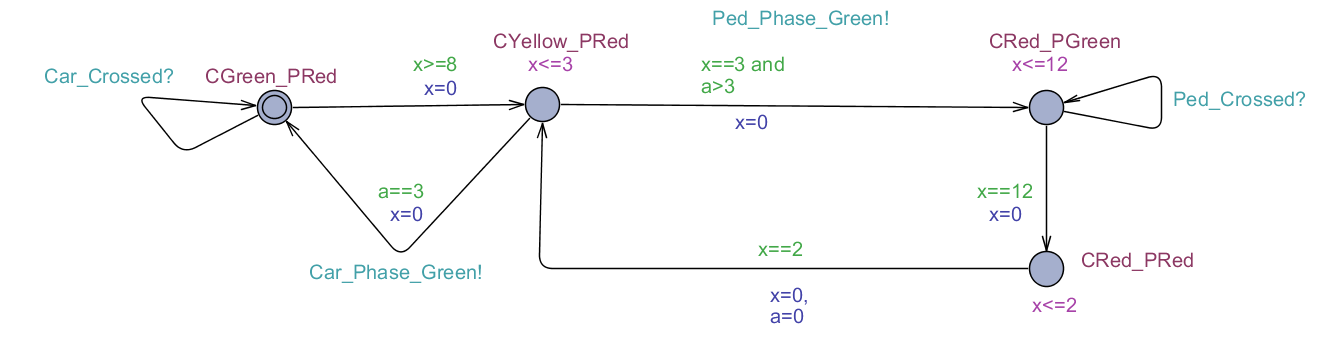
\includegraphics[width=\textwidth]{./UPAAAL_Screens/Contr1}
	\caption[Aufgabe 2i)]{Modell $Contr$ mit veränderten Time Constraints zur Verkürkung der Grünphase der Autos}    
\end{figure}

\begin{figure}[H] 
	\centering 
	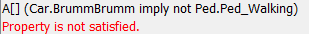
\includegraphics[width=0.5\textwidth]{./UPAAAL_Screens/2i_Verified}
	\caption[Aufgabe 2i)]{Verifizierungsergebnis der Propertie aus g) unter Verwendung der oben angegebenen alternativen Version von $Contr$}    
\end{figure}

Indem die Dauer der Rot/Grün, Rot/Rot und der Gelb/Rot Phasen auf insgesamt eine Sekunden verkürzt wurden, ist es möglich, dass die Grünphase der Autos nach einer Sekunde eintritt. Da der Fußgänger allerdings zwei bis drei Sekunden zum Überqueren der Straße benötigt, überschneiden sich die Übergangszeiten, wodurch das Modell nicht mehr sicher ist. 

\todo{Timing Constraints nochmal explizit angeben ? } 



\paragraph{j)}\mbox{} \\

Zwischen zwei grünen Amplephasen für Fußgäger liegen zwei mal die "'Dead Phase"', zwei mal die "'Yellow Phase"' und mindestens acht Sekunden grüne Ampelphase für die Autos, was insgesamt $2*2+2*3+8=18$ Sekunden ergibt, in dieser Zeit können nicht mehr als vier Fußgänger auftauchen, wenn sie alle fünf Sekunden auftauchen.
